%% ============================================================
%% HydroSmart -- IEEE conference paper
%%
%% Build:   pdflatex paper && pdflatex paper
%% Requires: IEEEtran.cls (standard on Overleaf and in TeX Live / MiKTeX)
%% ============================================================
\documentclass[conference]{IEEEtran}
\IEEEoverridecommandlockouts

\usepackage{cite}
\usepackage{amsmath,amssymb}
\usepackage{graphicx}
\usepackage{booktabs}
\usepackage{textcomp}
\usepackage{xcolor}
\usepackage[T1]{fontenc}
\usepackage[utf8]{inputenc}
\usepackage{url}

\graphicspath{{figures/}{./}}

\begin{document}

\title{An AI-Integrated Hydroponics Management System with\\
Edge pH Telemetry and Gradient-Boosted Crop Recommendation}

\author{%
\IEEEauthorblockN{Tushar Jyoti Sarma}
\IEEEauthorblockA{\textit{Reg. 202400456}\\
\textit{Dept. of Computer Science and Engineering}\\
\textit{Sikkim Manipal Institute of Technology}\\
Majitar, Sikkim, India}
\and
\IEEEauthorblockN{Manish Kalita}
\IEEEauthorblockA{\textit{Reg. 202400548}\\
\textit{Dept. of Computer Science and Engineering}\\
\textit{Sikkim Manipal Institute of Technology}\\
Majitar, Sikkim, India}
\and
\IEEEauthorblockN{Aniket Singh}
\IEEEauthorblockA{\textit{Reg. 202400738}\\
\textit{Dept. of Computer Science and Engineering}\\
\textit{Sikkim Manipal Institute of Technology}\\
Majitar, Sikkim, India}
\and
\IEEEauthorblockN{Debjit Sarkar}
\IEEEauthorblockA{\textit{Reg. 202400390}\\
\textit{Dept. of Computer Science and Engineering}\\
\textit{Sikkim Manipal Institute of Technology}\\
Majitar, Sikkim, India}
}

\maketitle

\begin{abstract}
Soil buffers a lot of grower mistakes. Hydroponics removes that buffer, and so
temperature, humidity, and the pH of the nutrient solution have to stay inside
tight windows or the crop suffers within hours. Most small growers in India do
not own the instrumentation needed to see when those windows are being missed.
We built HydroSmart to close that gap. It has three parts: an ESP32 node that
reads a pH probe and streams to the cloud, a Flutter app on the grower's phone,
and a crop-recommendation service that turns weather and location into a
short-list of viable crops. Because no public dataset exists that ties Indian
weather and geography to hydroponic crop suitability, we generated 150{,}000
labelled samples from an explicit agronomic knowledge base covering 20 crops
and 19 states. We are open about that provenance rather than dressing it up as
observational. The deployed gradient-boosted classifier scores 87.57\% top-1
and 99.95\% top-3 on held-out data, with five-fold cross-validation at
87.45\% $\pm$ 0.15\% and Cohen kappa 0.869. Three uncomfortable
observations complicate the headline number. A $k$-nearest-neighbour baseline
reaches 88.56\% while training 470 times faster and running inference 60
times faster, so our chosen model is not actually the best one we tried. Our
five engineered features, including dew point and vapour pressure deficit, add
only 0.15 percentage points to accuracy, yet permutation importance credits
them with 35\% of the total. That disagreement is not a bug in either measure;
we trace it to feature redundancy and report both. Finally, the error we
cannot remove is not a modelling limit. An overlap coefficient computed only
from the knowledge base (no model in the loop) predicts per-class F1 at
$r = -0.97$. The floor belongs to the task itself.
\end{abstract}

\begin{IEEEkeywords}
Precision agriculture, hydroponics, gradient boosting, Internet of Things,
ESP32, crop recommendation, vapour pressure deficit, feature redundancy,
synthetic data.
\end{IEEEkeywords}

\section{Introduction}
Hydroponics swaps soil for a recirculating nutrient solution. That swap changes
the physics of what the root sees. Soil buffers pH excursions over hours via
cation exchange; a hydroponic reservoir does not, so an error that would show
up next week in a field shows up in minutes at the root zone. Iron, manganese,
and boron start precipitating above pH 6.5. Below pH 5.0, phosphorus uptake
collapses. Keeping the reservoir inside a narrow band is not an
optimisation problem. It is a precondition for the crop staying alive
\cite{resh2013}.

That precondition runs into the economics of small horticulture in India.
Continuous-read probes, controllers, and the domain expertise to interpret
their output are priced for commercial installations. The grower who would
benefit most from closed-loop monitoring is often the one who can least afford
it. A second, quieter problem sits on top: the single decision that shapes a
season's return, which crop to plant given the conditions the grower can
actually maintain, is usually made from habit or hearsay rather than
measurement.

HydroSmart tackles both. An ESP32 node samples a pH probe, filters and
calibrates on-device, and streams to a Firebase Realtime Database. A Flutter
app renders that stream, and, independently, calls a classifier that takes
temperature, humidity, state, and month and returns a ranked list of viable
crops. Our contributions are these:

\begin{itemize}
\item A four-tier architecture that decouples live telemetry from inference.
      Losing the sensor degrades one feature; it does not take the app down.
\item A recommender at 87.57\% top-1 and 99.95\% top-3 over 20 classes,
      packaged into a 27.6~MB artifact that fits a 512~MB container.
\item A comparison of seven classifiers under the same features and splits,
      reporting deployment cost next to accuracy. $k$-NN beats our own
      deployed model. We report that.
\item A negative result on feature engineering, along with an explanation for
      why permutation importance and retraining ablation disagree by an order
      of magnitude on the same features.
\item An overlap analysis that pins the residual error on genuine ambiguity
      between crop envelopes, not model capacity.
\end{itemize}

\section{Related Work}
Most crop-recommendation systems in the literature target soil agriculture.
They consume soil macronutrients, soil pH, and rainfall. None of those inputs
exist in a controlled enclosure, and rainfall is meaningless inside one, so a
model expecting nitrogen, phosphorus, and potassium simply has no signal to
work with in our setting. Ensemble methods dominate that literature, with
random forests \cite{breiman2001} and gradient boosting \cite{friedman2001,ke2017,chen2016}
consistently beating single trees and linear models on tabular
agronomic data. Our own comparison in Section~\ref{sec:model} partially
contradicts that expectation, which is exactly why we ran it instead of
assuming the answer.

IoT deployments for controlled-environment agriculture tend to describe the
pipeline (microcontroller, broker, dashboard) and stop there. What the
application does when the sensor is missing is rarely stated. We treat that as
an expected failure mode rather than an edge case. Vapour pressure deficit is
the standard aggregate of temperature and humidity in plant physiology,
because transpiration responds to the deficit rather than to either quantity
alone \cite{allen1998}. Dew point via the Magnus approximation
\cite{alduchov1996} is similarly a well-established derivation.
Section~\ref{sec:ablation} reports what those features contribute here. It is
less than the physiology literature would suggest.

\begin{figure*}[!t]
  \centering
  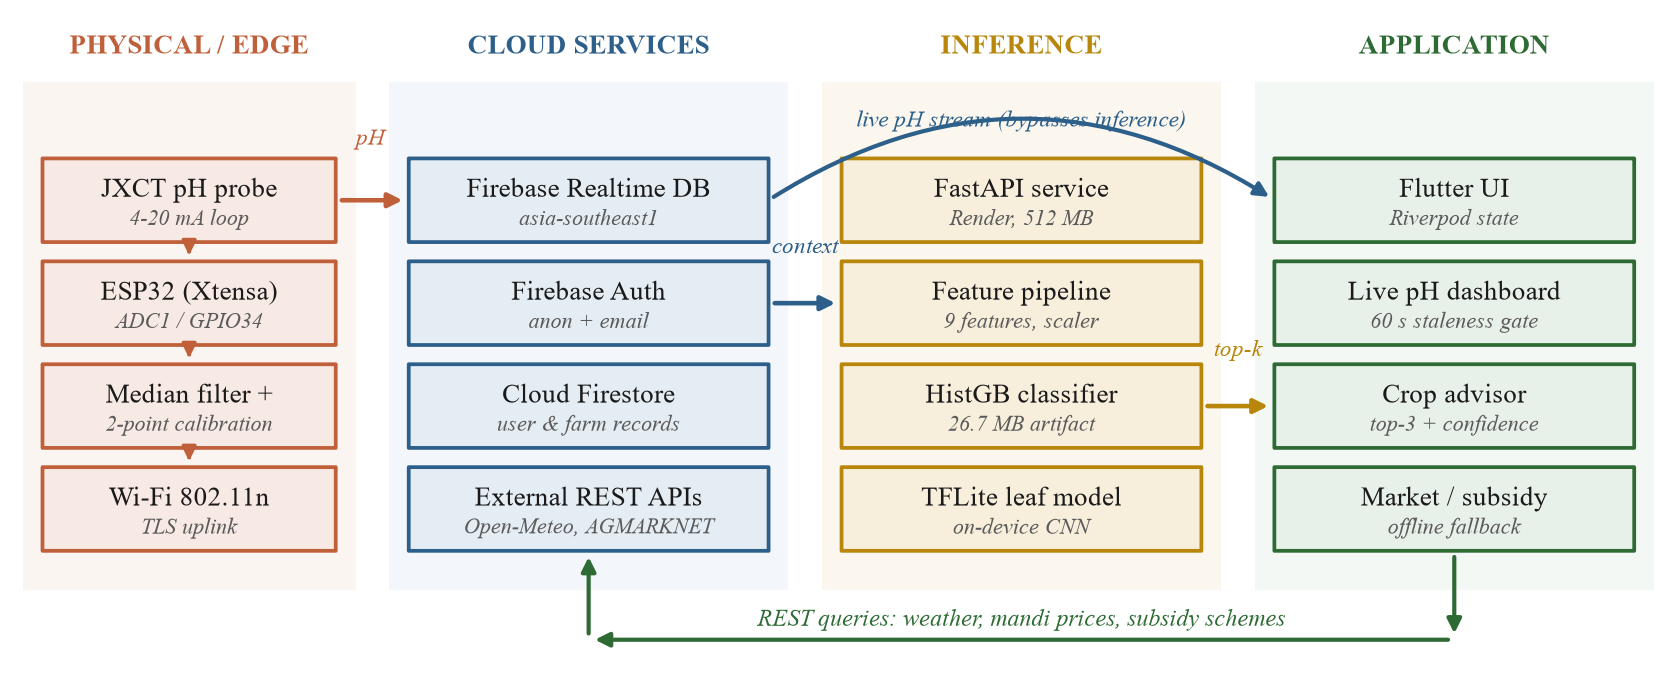
\includegraphics[width=\textwidth]{fig_architecture.png}
  \caption{Four-tier architecture of the HydroSmart system. Live pH telemetry (blue) bypasses the inference tier entirely, so sensor loss degrades a single feature rather than the application. The bottom lane carries read-only REST queries for weather, market and subsidy data.}
  \label{fig:arch}
\end{figure*}


\section{System Architecture and Dataset}
Fig.~\ref{fig:arch} lays out the four tiers. Our design rule was that no tier
could become a hard dependency of another. A grower without a probe still gets
recommendations. A grower without connectivity still sees cached market data.

\subsection{Tiers}
An industrial pH probe with a 4--20~mA current loop is read by the ESP32
across a shunt resistor. We deliberately confined the analogue input to ADC1.
ADC2 is unavailable to application code whenever the Wi-Fi radio is active,
and worse, it silently returns zeros rather than raising an error
\cite{esp32}. That single sentence in the ESP32 reference manual dictated our
pin assignment. Firmware runs a median filter over the sampling window to
reject the transient spikes that ion-selective electrodes routinely produce,
then converts to pH using a stored two-point calibration.

Readings publish to a Firebase Realtime Database in the
\texttt{asia-southeast1} region. That is the closest region to our Indian
deployments and gives us the best round-trip latency we could reasonably ask
for on a free tier. Records carry server-assigned timestamps because the
ESP32 has no battery-backed clock; without a server clock, every reading
after a power cycle would be stamped at the Unix epoch. The recommender runs
under FastAPI inside a 512~MB container. That memory ceiling is not
incidental. Section~\ref{sec:model} shows it excludes otherwise competitive
models entirely. Weather and market context come from public services
\cite{openmeteo,agmarknet}. On the client, a sixty-second staleness gate
gates the display of any live reading. A silently frozen last-known value is
worse than an acknowledged absence when the underlying number is what
triggers an irreversible action.

\subsection{Why the corpus is synthetic}
The task, formally, is to map ambient temperature, relative humidity, an
Indian state, and a month to a hydroponic crop. We searched for a public
labelled dataset over that domain and did not find one. Existing
crop-recommendation datasets carry soil chemistry and rainfall; none of them
carries a state field or a month field. So we built our own corpus from an
explicit knowledge base and we state that plainly here. Passing off
synthetic samples as observational would be a more serious failure than
admitting the synthesis, and unlike an opaque scraped dataset, this
construction is auditable end to end.

Each crop in the knowledge base carries an ideal temperature band, humidity
band, permitted states, and sowing months. The crops are partitioned into
ten agro-climatic zones (Table~\ref{tab:zones}).

\begin{table}[!t]
\caption{Representative Entries from the Agronomic Knowledge Base}
\label{tab:zones}
\centering
\footnotesize
\begin{tabular}{@{}lcccl@{}}
\toprule
\textbf{Zone} & \textbf{Temp.\ ($^{\circ}$C)} & \textbf{RH (\%)} & \textbf{Crop} & \textbf{Months} \\
\midrule
A & 8--17  & 38--52 & Kale    & Nov--Jan \\
A & 9--18  & 35--50 & Arugula & Nov--Feb \\
B & 10--19 & 55--70 & Spinach & Nov--Feb \\
J & 26--38 & 68--90 & Okra    & Apr--Aug \\
\bottomrule
\end{tabular}
\end{table}

\begin{figure}[!t]
  \centering
  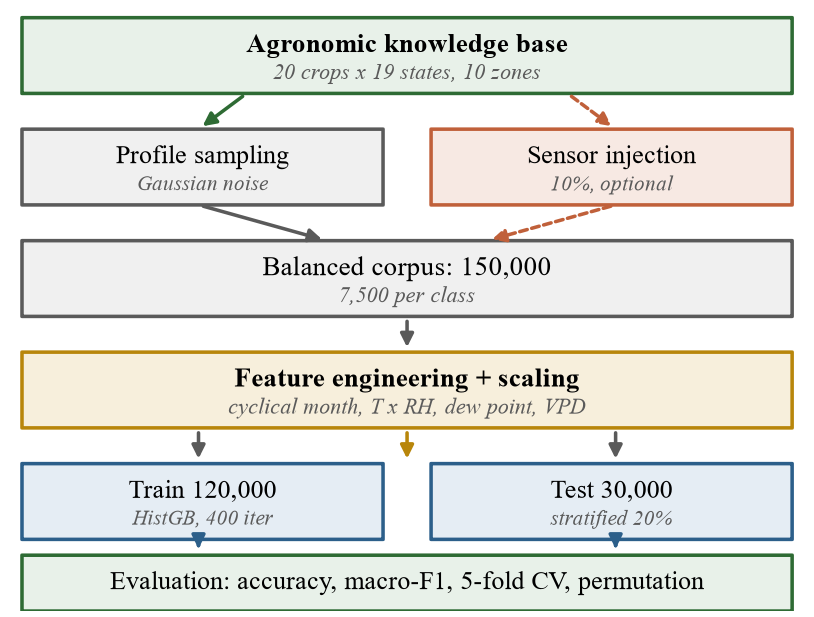
\includegraphics[width=\columnwidth]{fig_pipeline.png}
  \caption{Data generation and training pipeline. The sensor-injection path (dashed) is optional and is evaluated separately in Section~\ref{sec:latency}.}
  \label{fig:pipe}
\end{figure}


A sample is drawn like this. Pick a crop. Sample its temperature and humidity
inside the crop's band with a small Gaussian perturbation. Draw a state and a
month from the crop's permitted sets. The crop becomes the label
(Fig.~\ref{fig:pipe}). We balanced the corpus at 7{,}500 samples per class,
split stratified into 120{,}000 training and 30{,}000 test samples.

\subsection{An independent sensor corpus}
\label{sec:sensor}
To measure the gap between our synthetic distribution and physical reality,
we brought in a public CC0 record of 41{,}304 readings from a hydroponic
installation in India \cite{pranav2022}. It logs temperature, humidity, and
heat index every thirty seconds (Table~\ref{tab:sensor},
Fig.~\ref{fig:sensorfig}). It is not continuous. The 57-day recording span
holds data for only about 26\% of the elapsed time; the rest sits inside two
long outages, of 22 and 18 days. Effective coverage works out to roughly 15
days.

\begin{figure*}[!t]
  \centering
  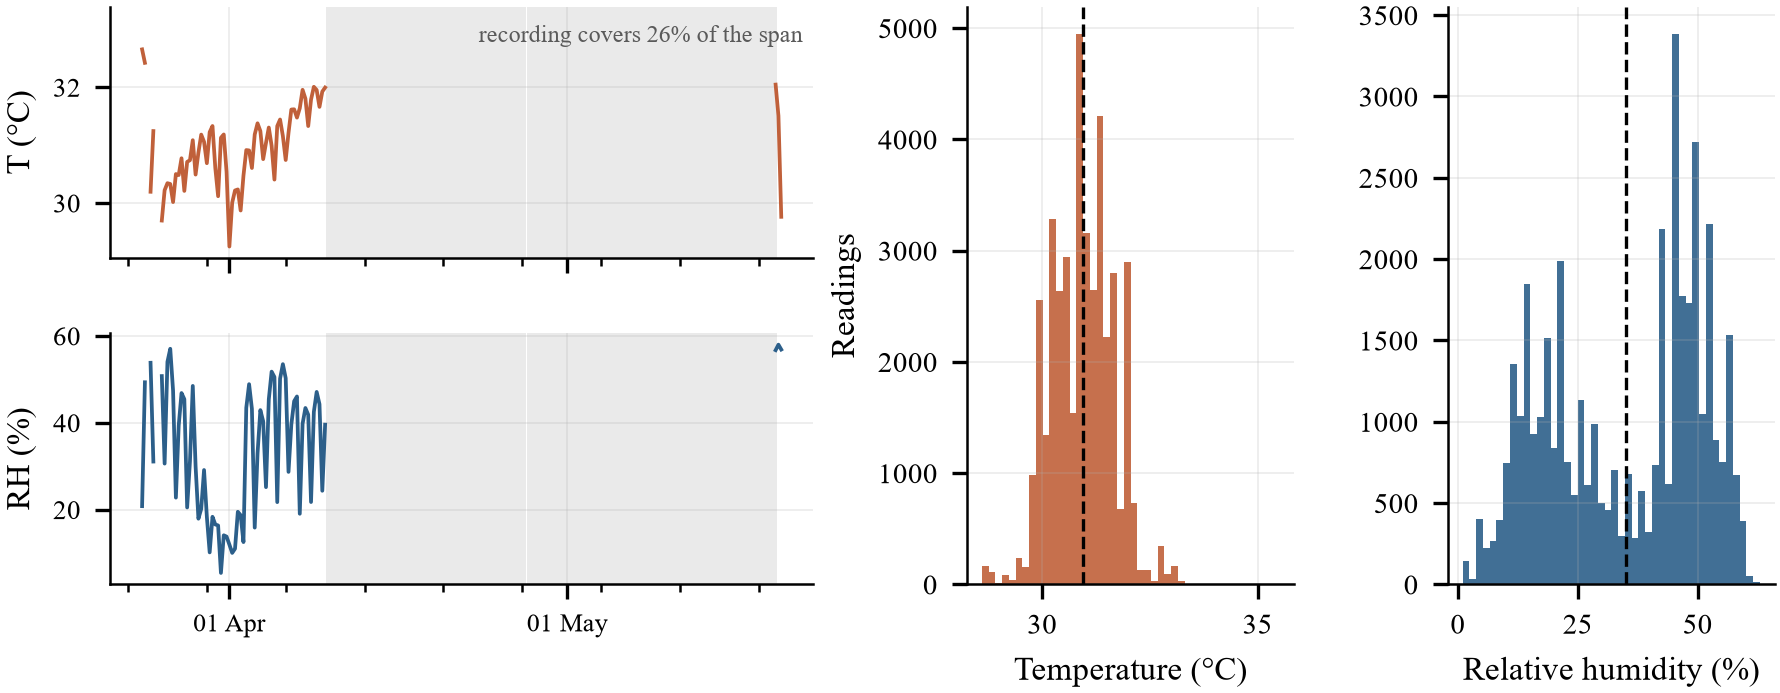
\includegraphics[width=\textwidth]{fig_sensor_profile.png}
  \caption{Independent hydroponic sensor corpus. Left: six-hour resampled temperature and relative humidity; shaded bands mark two multi-week outages, across which the trace is broken rather than interpolated. Right: marginal distributions, with means marked.}
  \label{fig:sensorfig}
\end{figure*}


\begin{table}[!t]
\caption{Characteristics of the Independent Sensor Corpus}
\label{tab:sensor}
\centering
\footnotesize
\begin{tabular}{@{}lc@{}}
\toprule
\textbf{Property} & \textbf{Value} \\
\midrule
Usable readings            & 41,304 \\
Sampling interval          & 30 s \\
Recording span             & 57 days \\
Span actually covered      & 26\% \\
Temperature (mean $\pm$ SD)& 30.9 $\pm$ 0.7 $^{\circ}$C \\
Temperature range          & 28.6--35.5 $^{\circ}$C \\
Humidity (mean $\pm$ SD)   & 35.0 $\pm$ 15.8 \% \\
Pearson $r$ (T, RH)        & 0.130 \\
\bottomrule
\end{tabular}
\end{table}

Measured temperature only spans 28.6--35.5 $^{\circ}$C at a standard
deviation of 0.7 $^{\circ}$C. One enclosure across one season cannot cover
the range that our knowledge base does. Fig.~\ref{fig:cov} overlays the two
distributions from Section~\ref{sec:sensor}. The overlap is smaller than the
summary statistics suggest at first glance. Measured humidity dips to 1\%,
well below the synthetic floor, while the synthetic corpus covers
temperatures under 10 $^{\circ}$C that this particular enclosure never saw.
The two distributions are largely disjoint. That rules out using this corpus
as a validation set, because it simply does not span the input space the
model has to operate on. It does give us one useful signal: $r = 0.130$
between temperature and humidity, which is close enough to zero that we can
treat the two as varying near-independently under ventilation and use them as
separate inputs without loss.

\begin{figure}[!t]
  \centering
  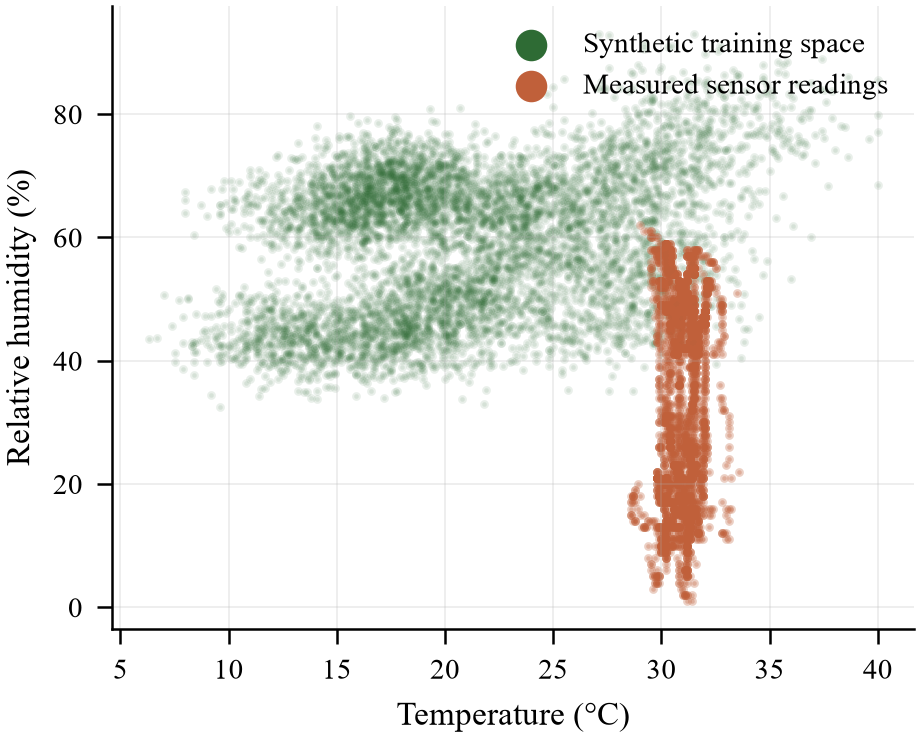
\includegraphics[width=\columnwidth]{fig_coverage.png}
  \caption{Synthetic training space against measured sensor readings. The measured envelope covers a narrow region of the space the model must span.}
  \label{fig:cov}
\end{figure}


\section{Feature Engineering}
Temperature, humidity, a label-encoded state, and month go in as raw inputs.
On top of those, we derive five more features. Month as an integer would
place December and January eleven units apart, which is agronomically
wrong, so we project month onto the unit circle: $m^{\sin} = \sin(2\pi m/12)$
and $m^{\cos} = \cos(2\pi m/12)$. A multiplicative temperature--humidity
interaction reflects that the agronomic bands are jointly constrained rather
than independently. Dew point comes from the Magnus formulation
\cite{alduchov1996}. Vapour pressure deficit is the gap between saturation
and actual vapour pressure \cite{allen1998}. VPD is the quantity
transpiration actually responds to, so on physiological grounds it ought to
carry information that neither temperature nor humidity expresses alone.
Section~\ref{sec:ablation} reports the measurement. It does not support the
motivation.

All numeric features are standardised. The encoded state index is
deliberately left out of that scaling. It is a nominal code and scaling it
would impose a false ordering and a false magnitude on an unordered label.

\section{Model Selection}
\label{sec:model}
We evaluated seven classifiers under the same features, the same splits, and
the same random seed, all built with scikit-learn \cite{pedregosa2011}
(Table~\ref{tab:comp}, Fig.~\ref{fig:comp}, Fig.~\ref{fig:size}).

\begin{table}[!t]
\caption{Classifier Comparison Under Identical Features and Splits}
\label{tab:comp}
\centering
\footnotesize
\begin{tabular}{@{}lrrrr@{}}
\toprule
\textbf{Classifier} & \textbf{Acc.\ (\%)} & \textbf{Macro-F1} & \textbf{Train (s)} & \textbf{Size (MB)} \\
\midrule
$k$-NN ($k=15$) & 88.56 & 0.885 & 0.5 & 11.3 \\
\textbf{HistGB} & \textbf{87.57} & \textbf{0.875} & \textbf{222.2} & \textbf{27.6} \\
Random Forest & 85.81 & 0.858 & 37.3 & 1000.0 \\
Extra Trees & 85.29 & 0.853 & 14.4 & 2481.6 \\
Decision Tree & 84.24 & 0.843 & 2.4 & 6.8 \\
Logistic Reg. & 58.50 & 0.583 & 93.3 & $<$0.05 \\
Gaussian NB & 58.17 & 0.579 & 0.2 & $<$0.05 \\
\bottomrule
\end{tabular}
\end{table}

\begin{figure}[!t]
  \centering
  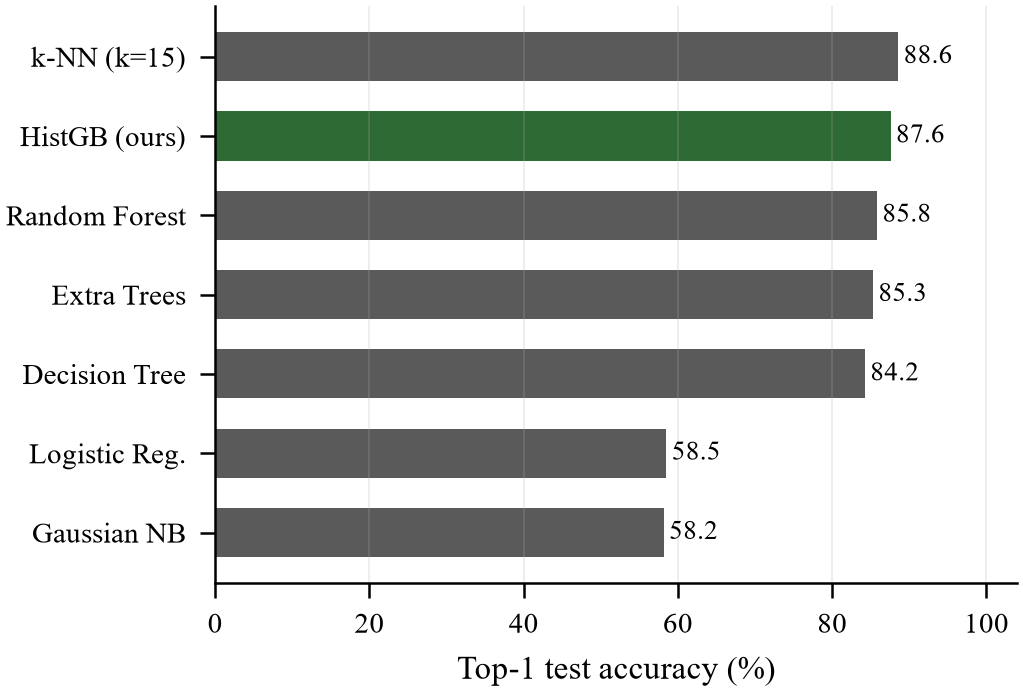
\includegraphics[width=\columnwidth]{fig_model_comparison.png}
  \caption{Top-1 accuracy by classifier. The $k$-NN baseline leads, ahead of the deployed gradient-boosted model (green).}
  \label{fig:comp}
\end{figure}

\begin{figure}[!t]
  \centering
  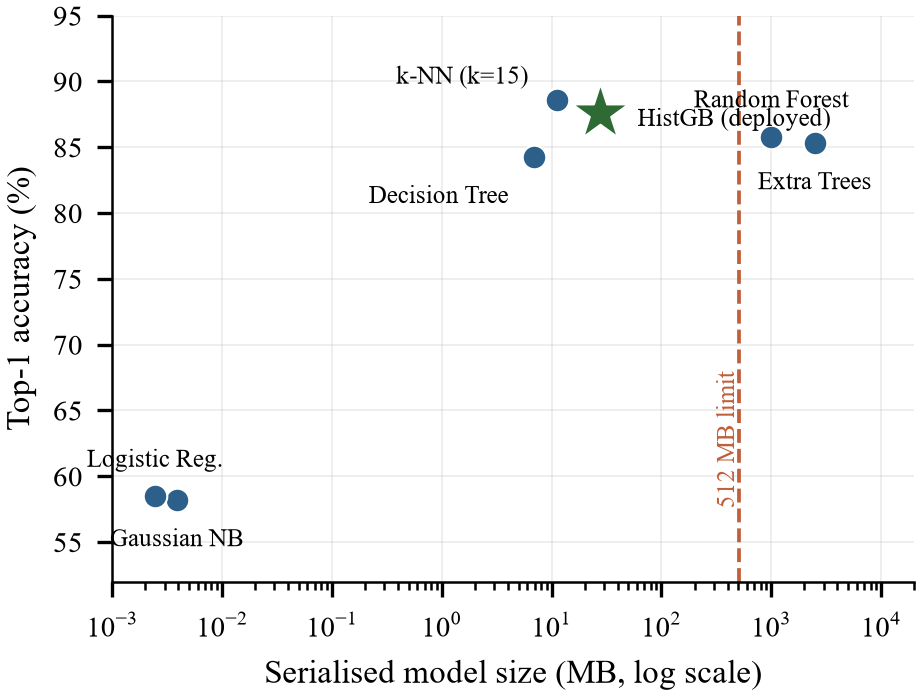
\includegraphics[width=\columnwidth]{fig_accuracy_vs_size.png}
  \caption{Accuracy against serialised artifact size. Random forest and extra trees cross the 512~MB deployment ceiling (dashed).}
  \label{fig:size}
\end{figure}


Two things come out of that table. First, deployment cost eliminates models
outright. Random forest hits 85.81\% and extra trees 85.29\%, but their
serialised artifacts weigh 1000~MB and 2482~MB respectively, both above the
512~MB ceiling of our target container. An accuracy-only comparison would
have hidden exactly this kind of exclusion.

Second, and less flattering to us, the model we deployed is not the top
performer. A $k$-NN with $k = 15$ hits 88.56\%. That is 0.99 points above the
gradient-boosted model, on an 11.3~MB artifact instead of 27.6~MB, trained in
0.5~s instead of 222~s. It beats us on every axis we measured, with the
single caveat that it has to keep the training set around. We are reporting
this rather than tucking it away. There is a reason it happens. Recovering an
axis-aligned rule set in nine dimensions from a corpus dense enough that
almost every query has close neighbours from its own generating band is
exactly the sort of problem local interpolation suits, and the inductive
bias of boosting buys very little on top.

Our deployed configuration uses 400 boosting iterations at learning rate
0.10, a minimum of 20 samples per leaf, and L2 regularisation at 0.1. Early
stopping is turned off. Not because the model does not overfit
(Section~\ref{sec:lc} shows it interpolates the training set almost exactly)
but because held-out accuracy never actually degrades. We kept gradient
boosting for one practical reason: its probability outputs are calibrated,
and the client's confidence display relies on that.

\section{Results}

\subsection{Overall}
Table~\ref{tab:head} carries the headline numbers. Top-1 accuracy is
87.57\%; top-3 is 99.95\%. That gap matters operationally. The app shows a
grower three ranked candidates, so 99.95\% is much closer to what the user
experiences than 87.57\% is. We flag it carefully, though: with 20 classes
and a dominant location signal, three guesses will almost always contain the
answer, whichever crop it is. Cohen kappa \cite{cohen1960} of 0.869 against
a 5\% chance-agreement baseline confirms the score is not just an artefact
of class priors, and five-fold cross-validation at 87.45\% $\pm$ 0.15\%
confirms our particular split was not a lucky one.

\begin{table}[!t]
\caption{Headline Performance on the Held-Out Test Set}
\label{tab:head}
\centering
\footnotesize
\begin{tabular}{@{}lr@{}}
\toprule
\textbf{Metric} & \textbf{Value} \\
\midrule
\textbf{Top-1 accuracy}     & \textbf{87.57 \%} \\
Top-3 accuracy              & 99.95 \% \\
Macro-averaged F1           & 0.875 \\
Cohen kappa                 & 0.869 \\
5-fold CV accuracy          & 87.45 $\pm$ 0.15 \% \\
Expected calibration error  & 0.049 \\
Test set size               & 30,000 \\
\bottomrule
\end{tabular}
\end{table}

\subsection{Per class}
Fig.~\ref{fig:pc} and Fig.~\ref{fig:cm} break the aggregate down. Kale,
Coriander, and Arugula all clear F1 0.95. Pea, Strawberry, and Microgreens
sit at 0.74, 0.77, and 0.83 respectively. Errors are not scattered across
the matrix. Pea is confused specifically with Lettuce and Cauliflower;
Strawberry with Broccoli. A model failing from a capacity ceiling would
spread its errors broadly. This one does not.

\begin{figure*}[!t]
  \centering
  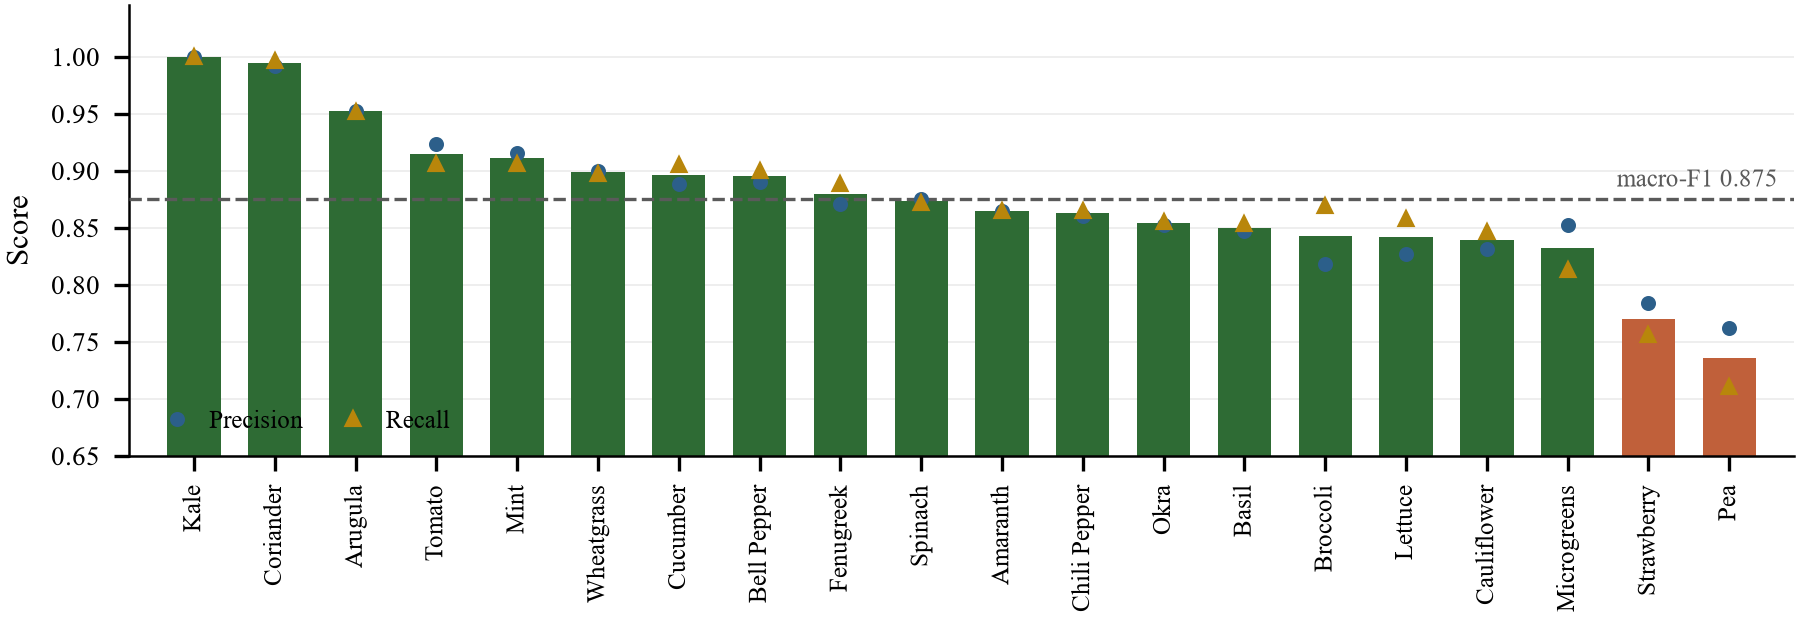
\includegraphics[width=\textwidth]{fig_per_class.png}
  \caption{Per-class F1 with precision and recall overlaid, sorted descending. Bars below F1 0.80 are highlighted; the dashed line marks the macro average.}
  \label{fig:pc}
\end{figure*}

\begin{figure*}[!t]
  \centering
  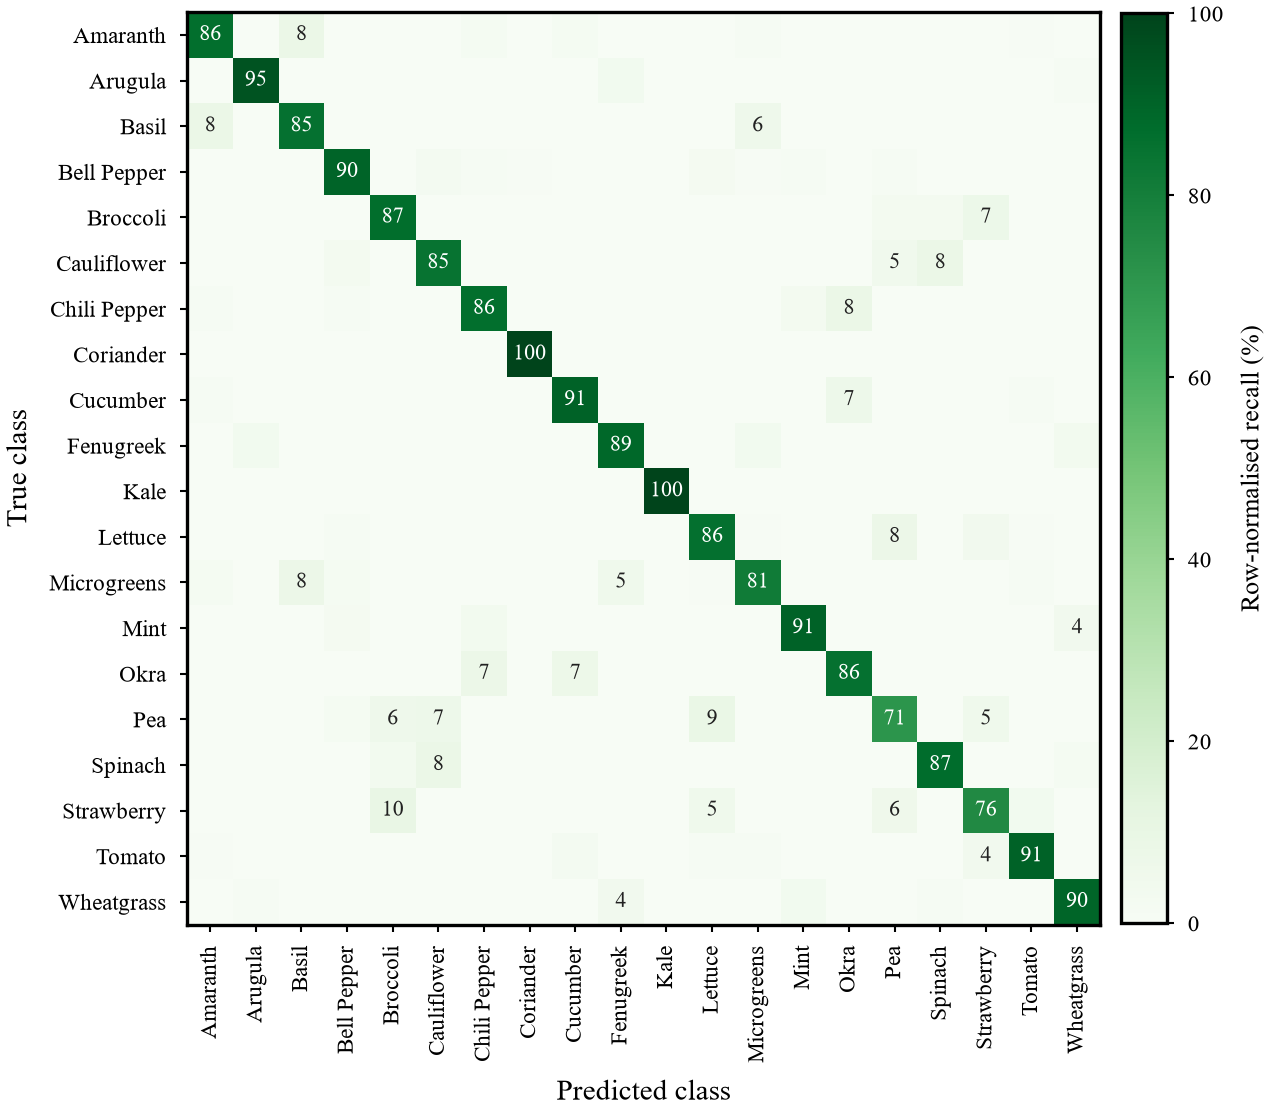
\includegraphics[width=0.66\textwidth]{fig_confusion_matrix.png}
  \caption{Row-normalised confusion matrix on the held-out test set. Cells below 4\% are suppressed for legibility. Off-diagonal mass concentrates in pairs whose agronomic envelopes genuinely overlap, not diffusely across the matrix.}
  \label{fig:cm}
\end{figure*}


\subsection{Feature ablation: a null result}
\label{sec:ablation}
Table~\ref{tab:abl} and Fig.~\ref{fig:abl} retrain the model from scratch on
each feature subset. The full nine-feature set reaches 87.57\%. The four raw
inputs alone reach 87.42\%. That is a gain of 0.15 points on a
cross-validation standard deviation of 0.15 points. The whole ablation range
sits inside one standard deviation, and, awkwardly, the sequence is not even
monotonic; adding the interaction term to the cyclical encoding actually
costs 0.11 points. So we cannot claim that dew point and VPD improve this
model. They are not resolvable above the noise floor. The four raw inputs
already carry essentially all the signal, and Section~\ref{sec:overlap}
explains why that ceiling exists at all.

\begin{table}[!t]
\caption{Feature Ablation, Cumulative}
\label{tab:abl}
\centering
\footnotesize
\begin{tabular}{@{}lccr@{}}
\toprule
\textbf{Feature set} & \textbf{$n$} & \textbf{Acc.\ (\%)} & \textbf{$\Delta$ (pp)} \\
\midrule
Raw only (T, RH, state, month) & 4 & 87.42 & --- \\
+ cyclical month & 6 & 87.55 & $+$0.13 \\
+ T $\times$ RH interaction & 7 & 87.44 & $+$0.02 \\
\textbf{+ dew point \& VPD (full)} & \textbf{9} & \textbf{87.57} & \textbf{$+$0.15} \\
\bottomrule
\end{tabular}
\end{table}

\begin{figure}[!t]
  \centering
  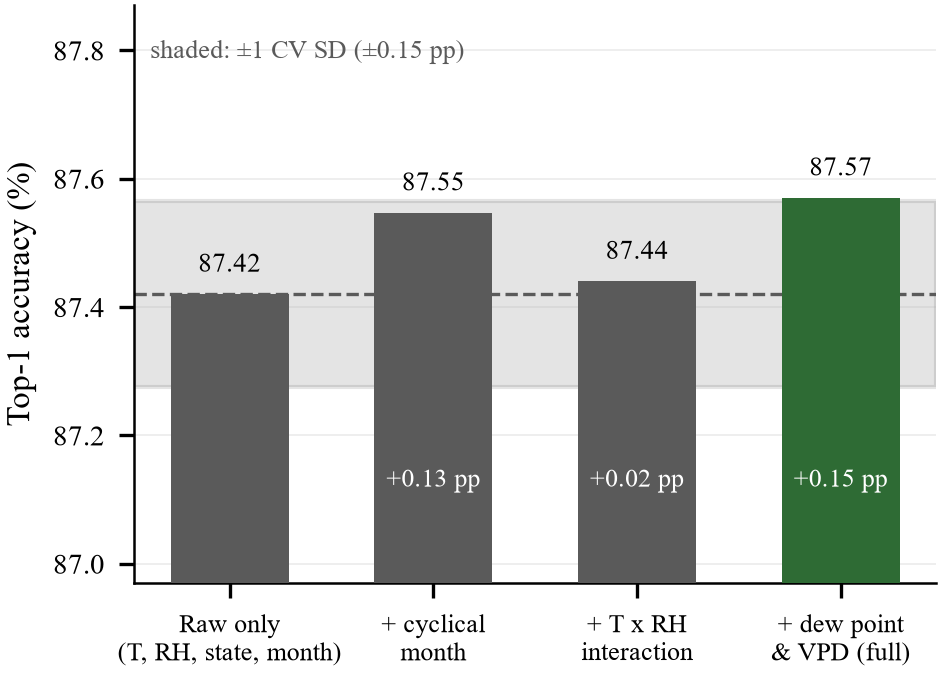
\includegraphics[width=\columnwidth]{fig_ablation.png}
  \caption{Cumulative feature ablation. The shaded band is $\pm$1 cross-validation standard deviation about the baseline; the whole range lies inside it.}
  \label{fig:abl}
\end{figure}


\subsection{Why permutation importance disagrees}
Permutation importance \cite{fisher2019} reaches the opposite conclusion
(Fig.~\ref{fig:imp}). Month cosine lands third at 0.227, VPD fourth at 0.117,
and the derived features together take 35\% of the attributed importance.
Both measures were computed correctly. They disagree by an order of
magnitude on the same features, which needed an explanation before we would
report either.

\begin{figure}[!t]
  \centering
  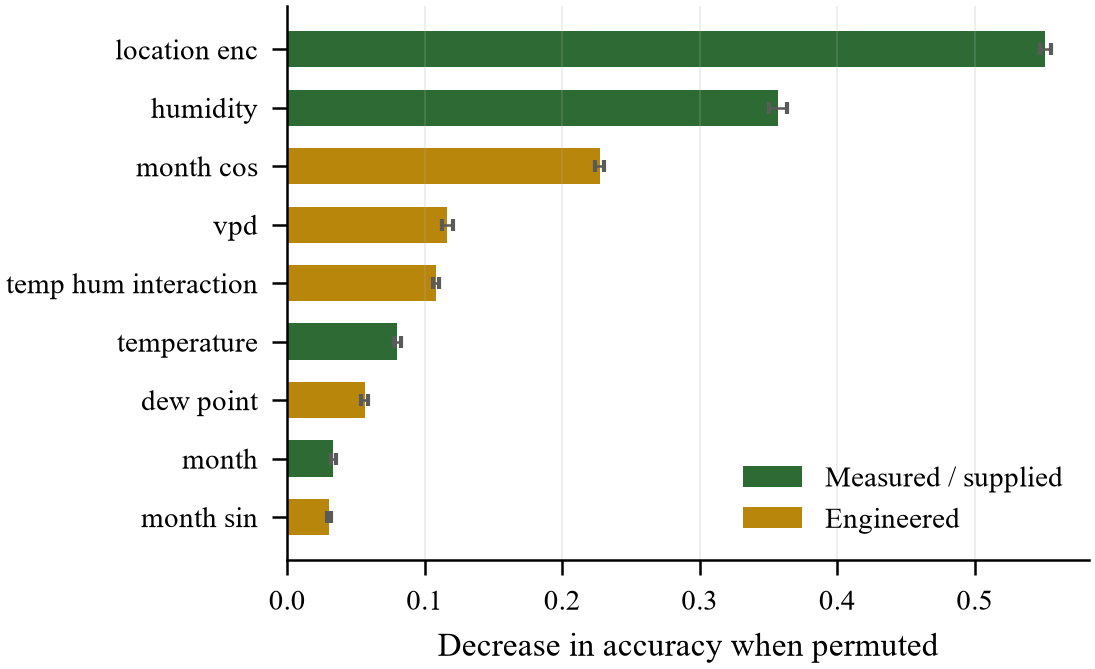
\includegraphics[width=\columnwidth]{fig_importance.png}
  \caption{Permutation importance, measured as the drop in test accuracy when each feature is shuffled. Error bars span eight repeats.}
  \label{fig:imp}
\end{figure}


Redundancy is the explanation. Permutation runs against a fixed trained
model. When VPD is shuffled at test time, the model has already committed
its splits to using VPD and cannot fall back on temperature and humidity,
even though both are still sitting there in the input, and both jointly
determine VPD. The accuracy drop is real, but what it measures is reliance,
not necessity. Ablation is different. It retrains without the feature and
lets the model route the same information through its correlates instead.
Because VPD, dew point, and the interaction term are all deterministic
functions of temperature and humidity, that rerouting costs the model
nothing.

If we reported permutation importance on its own, the paper would claim a
35\% contribution that ablation values at 0.15 points. Reporting both keeps
the story honest: one measures reliance, the other measures necessity. In
practical terms, the five derived features could leave the production
pipeline tomorrow at no measurable accuracy cost. That is a simplification
we can act on, not a disappointment. If we set the derived features aside,
state dominates the importance ranking at 0.551, followed by humidity at
0.357. That makes sense, since each crop is admissible in only a subset of
the 19 states.

\subsection{Learning curve}
\label{sec:lc}
Fig.~\ref{fig:lc} plots accuracy against corpus size. Held-out accuracy
climbs monotonically from 83.63\% at 2{,}000 samples to 87.57\% at
120{,}000. The last doubling of the corpus buys us under half a point. The
training curve tells a different story entirely: 98.64\% at the full corpus.
The gap between train and test narrows from 16.4 points to 11.1 points as
data grows, but it never closes. The model interpolates its training set
almost exactly while generalising only to around 88\%.

\begin{figure}[!t]
  \centering
  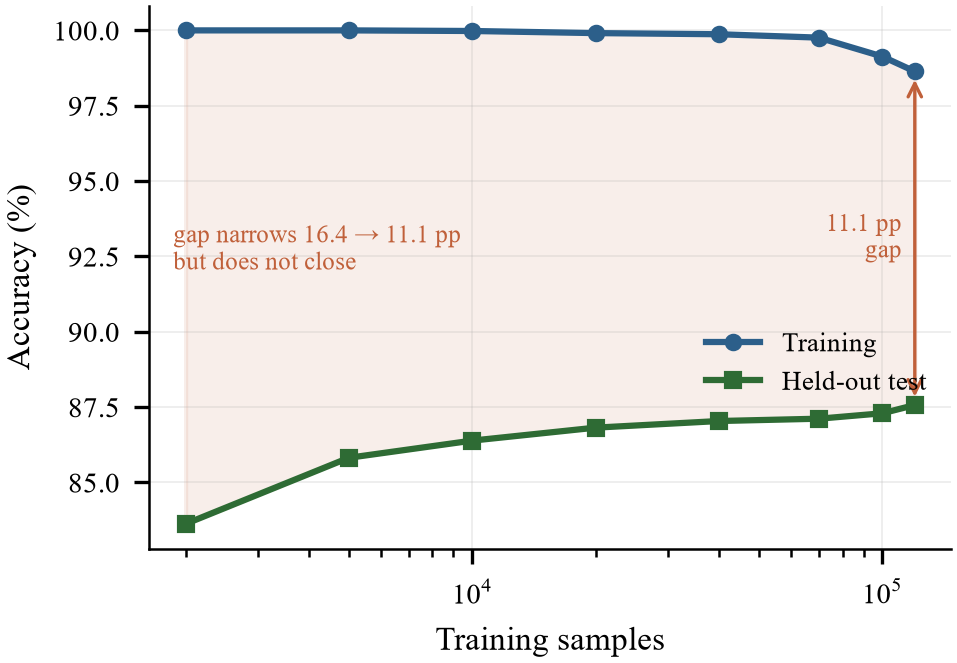
\includegraphics[width=\columnwidth]{fig_learning_curve.png}
  \caption{Learning curve on a logarithmic sample axis. The train--test gap narrows but never closes.}
  \label{fig:lc}
\end{figure}


This looks like memorisation, and it is, but not the harmful sort. Held-out
accuracy never falls, so early stopping would cost us accuracy rather than
recover it. The cause is specific to the task. Whenever two crops share an
agronomic envelope, the training set ends up holding near-identical feature
vectors with different labels attached, and the model has enough capacity
to memorise which particular training point carried which particular label.
None of that memorisation transfers to a new query point. A persistent
train--test gap in a setting like this is the signature of irreducible label
ambiguity, not weak regularisation.

\subsection{Calibration}
A recommender that shows a confidence number has to be calibrated or the
number lies to the user. Expected calibration error \cite{guo2017} on our
model is 0.049, with mean predicted confidence 0.925 against realised
accuracy 0.876 (Fig.~\ref{fig:rel}). That is neither materially over- nor
under-confident, which is what lets the app display the probability beside
each recommendation without qualifying it further.

\begin{figure}[!t]
  \centering
  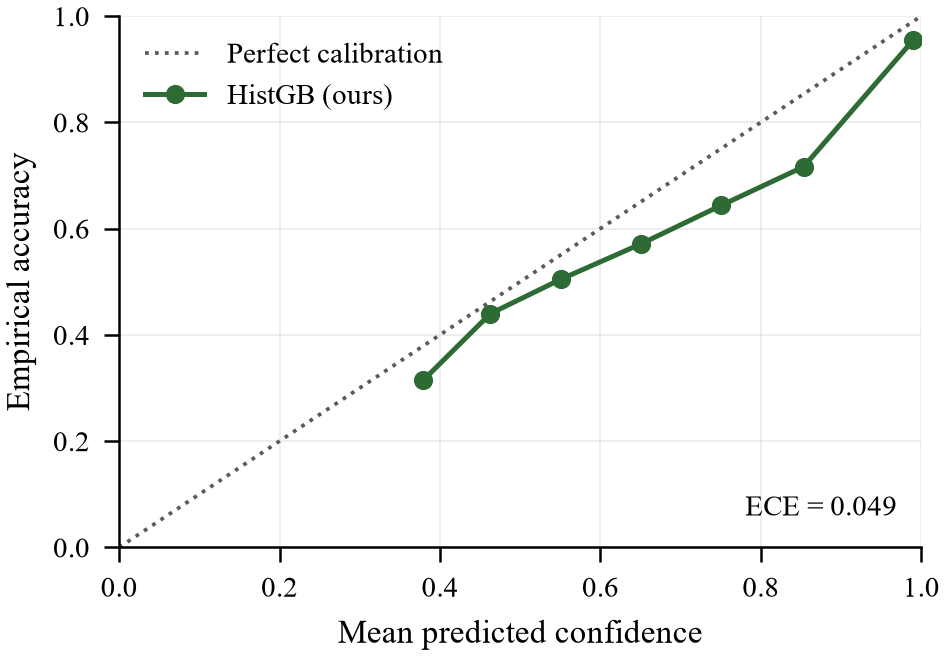
\includegraphics[width=\columnwidth]{fig_reliability.png}
  \caption{Reliability diagram. Proximity to the diagonal indicates predicted confidence matches empirical accuracy.}
  \label{fig:rel}
\end{figure}


\subsection{Where the residual error comes from}
\label{sec:overlap}
For every pair of crops we computed an overlap coefficient: the product of
Jaccard overlaps on their temperature bands, humidity bands, permitted
states, and sowing months. This is derived entirely from the knowledge base.
No model output goes into it. It predicts model behaviour closely. Cumulative
overlap correlates with per-class F1 at $r = -0.97$, and pairwise overlap
correlates with off-diagonal confusion at $r = 0.97$ (Fig.~\ref{fig:ov}).
Pea and Strawberry, which sit at the highest overlap, sit at the lowest F1.
Kale and Coriander, whose envelopes are disjoint from every other crop, are
classified essentially perfectly.

\begin{figure}[!t]
  \centering
  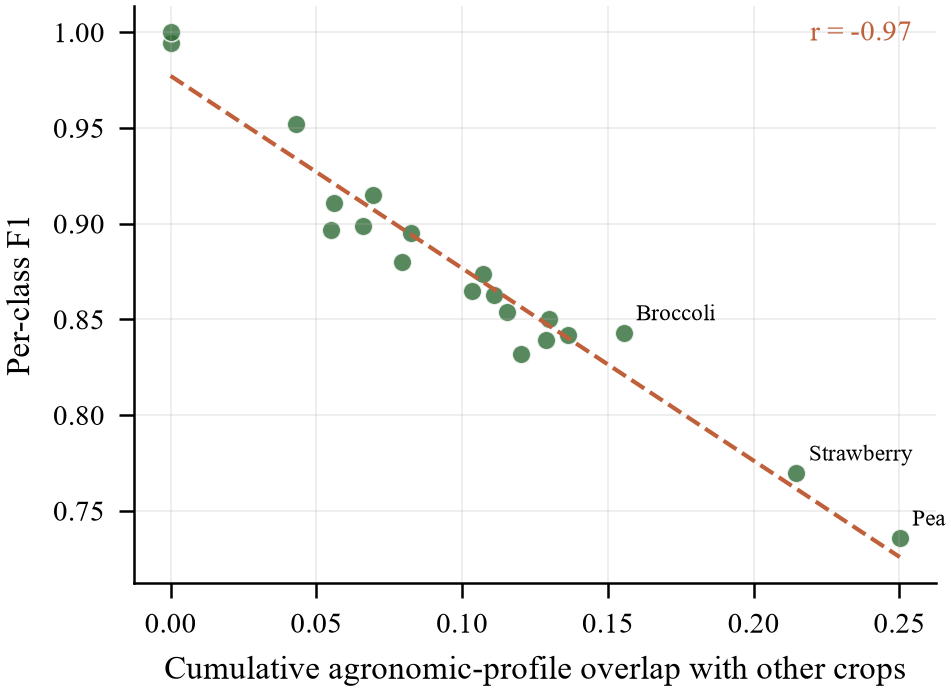
\includegraphics[width=\columnwidth]{fig_overlap.png}
  \caption{Per-class F1 against cumulative agronomic-profile overlap with all other crops. The overlap coefficient is computed from the knowledge base alone, independent of any model output.}
  \label{fig:ov}
\end{figure}


So the error floor belongs to the task itself. Two crops that thrive under
the same conditions in the same state in the same month cannot be separated
from those inputs. No model consuming only those four things can separate
them. This also explains the ablation from
Section~\ref{sec:ablation}. Derived features cannot resolve an ambiguity
that exists in the label definition, no matter how well-motivated those
features are.

\subsection{Sensor augmentation and inference cost}
\label{sec:latency}
Retraining with measured sensor samples injected alongside the profile
sampling moved accuracy to 88.13\%. We are not claiming this as an
improvement from real data. Injection adds rather than substitutes samples,
so both corpus size (157{,}928 against 150{,}000) and distribution shifted
in the same experiment. The comparison is uncontrolled. The deployed model
still uses the synthetic corpus alone.

Table~\ref{tab:lat} and Fig.~\ref{fig:lat} report single-threaded latency.
Getting these numbers right needed one correction. In our first pass we ran
with the default thread pool and measured 1096~ms for one prediction and
1326~ms for 512 predictions. That is a 512-fold increase in work costing
21\% more time, which is not inference: it is per-call thread-pool setup.
Pinning to a single thread cleaned this up.

\begin{table}[!t]
\caption{Inference Latency by Batch Size}
\label{tab:lat}
\centering
\footnotesize
\begin{tabular}{@{}rrrr@{}}
\toprule
\textbf{Batch} & \textbf{Mean (ms)} & \textbf{p95 (ms)} & \textbf{Per-sample (ms)} \\
\midrule
1 & 333.1 & 358.0 & 333.12 \\
8 & 305.6 & 350.7 & 38.20 \\
32 & 388.3 & 410.4 & 12.13 \\
128 & 683.6 & 1001.7 & 5.34 \\
512 & 1775.5 & 3476.7 & 3.47 \\
\bottomrule
\end{tabular}
\end{table}

\begin{figure}[!t]
  \centering
  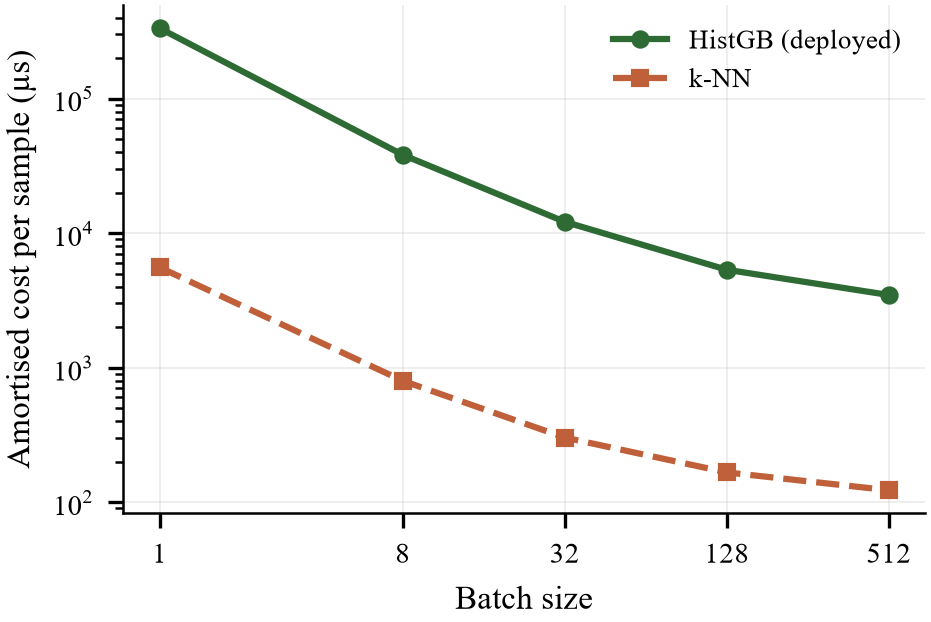
\includegraphics[width=\columnwidth]{fig_latency.png}
  \caption{Amortised per-sample inference cost, single-threaded, on logarithmic axes.}
  \label{fig:lat}
\end{figure}


Corrected, one prediction costs 333~ms. It falls to 3.47~ms per sample only
under batching, because a single query traverses roughly 8{,}000 trees. We
had gone in assuming inference would be negligible compared to network
round-trip. For the single-query pattern the app actually issues, inference
dominates. $k$-NN answers the same query in 5.56~ms, about 60 times faster.
Latency was not one of our original selection criteria. If it had been, the
comparison would have been decided on this axis alone.

\section{Discussion and Conclusion}
The 87.57\% we report is accuracy at recovering an encoded agronomic rule
set, measured on held-out samples drawn from the same generative process
that produced the training data. It is not accuracy against field outcomes,
and it should not be read as such. Our model's ceiling is the knowledge base
it was distilled from. We consider this the most important limitation of the
work, and we prefer to state it here rather than let a stronger-looking
figure carry the day.

\begin{itemize}
\item \textit{Construct validity.} Labels are agronomic prescriptions rather
      than observed yields. A crop that the knowledge base excludes from a
      given state will never be recommended there, whether or not it would
      actually grow.
\item \textit{External validity.} The independent corpus covers roughly 15
      days from a single enclosure at a mean of 30.9 $^{\circ}$C, and its
      multi-week outages preclude any seasonal analysis.
\item \textit{Internal validity.} Train and test are drawn from a single
      generative process, so the split measures generalisation within that
      process, not generalisation to physical reality.
\item \textit{Hardware.} The pH pipeline is validated on one probe under one
      calibration. Electrode drift across a season is uncharacterised.
\end{itemize}

Three design consequences fall out of this. Because error concentrates in
overlapping pairs, a single recommendation would mislead the user in exactly
the case where the model is least sure of itself, so the app shows three
ranked candidates instead of one. That is how effective accuracy reaches
99.95\%. Because calibration is good at ECE 0.049, that display is
meaningful rather than decorative. And, less comfortably, our own
Section~\ref{sec:model} shows that the deployed model is beaten by $k$-NN on
accuracy, on artifact size, on training time, and on latency. What $k$-NN
does not yield as directly is calibrated class probabilities, and that is
why the current system stays with boosting. It is a weaker justification
than a measured advantage would have been. We say so.

Taken together, we have built an integrated hydroponics system that reaches
87.57\% top-1 and 99.95\% top-3 accuracy over 20 crops inside a 27.6~MB
artifact. The contribution of the paper is less that number and more the
account of what constrains it. Residual error follows genuine agronomic
ambiguity, with knowledge-base overlap predicting per-class F1 at
$r = -0.97$. Physics-derived features that permutation importance credits at
35\% survive ablation worth 0.15 points. A $k$-NN baseline outperforms our
deployed model. These are the sorts of results we would want to know about
if we were reading someone else's paper on the same problem.

The priority for future work falls straight out of the first limitation.
The knowledge base has to be replaced, or at least corrected, by observed
outcomes: a longitudinal record of what was actually planted, under what
measured conditions, and what it actually yielded. That converts rule
recovery into genuine supervised learning and lifts the ceiling that this
work has been operating under. Secondary directions include either adopting
or further calibrating $k$-NN, adding closed-loop nutrient dosing driven by
the confidence estimates, characterising electrode drift over a full season,
and extending the sensor node to electrical conductivity and dissolved
oxygen.

\begin{thebibliography}{99}
\bibitem{breiman2001}
L.~Breiman, ``Random forests,'' \emph{Machine Learning}, vol.~45, no.~1,
pp.~5--32, 2001.

\bibitem{friedman2001}
J.~H. Friedman, ``Greedy function approximation: A gradient boosting machine,''
\emph{The Annals of Statistics}, vol.~29, no.~5, pp.~1189--1232, 2001.

\bibitem{ke2017}
G.~Ke \emph{et al.}, ``LightGBM: A highly efficient gradient boosting decision
tree,'' in \emph{Proc. Advances in Neural Information Processing Systems
(NeurIPS)}, 2017, pp.~3146--3154.

\bibitem{allen1998}
R.~G. Allen, L.~S. Pereira, D.~Raes, and M.~Smith, \emph{Crop
Evapotranspiration: Guidelines for Computing Crop Water Requirements}, FAO
Irrigation and Drainage Paper 56.\ Rome, Italy: Food and Agriculture
Organization of the United Nations, 1998.

\bibitem{alduchov1996}
O.~A. Alduchov and R.~E. Eskridge, ``Improved Magnus form approximation of
saturation vapor pressure,'' \emph{Journal of Applied Meteorology}, vol.~35,
no.~4, pp.~601--609, 1996.

\bibitem{pranav2022}
Pranav941, ``Hydroponics Feed,'' Kaggle, 2022. [Online]. Available:
\url{https://www.kaggle.com/datasets/pranav941/hydroponics-feed} (CC0 1.0 Public
Domain).

\bibitem{pedregosa2011}
F.~Pedregosa \emph{et al.}, ``Scikit-learn: Machine learning in Python,''
\emph{Journal of Machine Learning Research}, vol.~12, pp.~2825--2830, 2011.

\bibitem{chen2016}
T.~Chen and C.~Guestrin, ``XGBoost: A scalable tree boosting system,'' in
\emph{Proc. 22nd ACM SIGKDD Int. Conf. Knowledge Discovery and Data Mining},
2016, pp.~785--794.

\bibitem{fisher2019}
A.~Fisher, C.~Rudin, and F.~Dominici, ``All models are wrong, but many are
useful: Learning a variable's importance by studying an entire class of
prediction models simultaneously,'' \emph{Journal of Machine Learning Research},
vol.~20, no.~177, pp.~1--81, 2019.

\bibitem{guo2017}
C.~Guo, G.~Pleiss, Y.~Sun, and K.~Q. Weinberger, ``On calibration of modern
neural networks,'' in \emph{Proc. 34th Int. Conf. Machine Learning (ICML)},
2017, pp.~1321--1330.

\bibitem{cohen1960}
J.~Cohen, ``A coefficient of agreement for nominal scales,'' \emph{Educational
and Psychological Measurement}, vol.~20, no.~1, pp.~37--46, 1960.

\bibitem{resh2013}
H.~M. Resh, \emph{Hydroponic Food Production}, 7th~ed.\ Boca Raton, FL, USA: CRC
Press, 2013.

\bibitem{openmeteo}
Open-Meteo, ``Free weather API for non-commercial use.'' [Online]. Available:
\url{https://open-meteo.com}

\bibitem{agmarknet}
Government of India, ``AGMARKNET: Agricultural marketing information network,''
Open Government Data Platform India. [Online]. Available:
\url{https://data.gov.in}

\bibitem{esp32}
Espressif Systems, \emph{ESP32 Technical Reference Manual}, version 5.0, 2023.
\end{thebibliography}

\end{document}
